\documentclass{beamer}

% You can also use a 16:9 aspect ratio:
%\documentclass[aspectratio=169]{beamer}
\usetheme{TACC16}

% It's possible to move the footer to the right:
%\usetheme[rightfooter]{TACC16}

\begin{document}
\title[Lmod]{SC18: 8th Annual Lmod Booth Talk}
\author{Robert McLay} 
\date{November 13, 2018} 

% page 1
\frame{\titlepage} 

\section{Introduction}

\begin{frame}{Introduction}
  \begin{itemize}
    \item Welcome to the 8th annual TACC Booth Talk
    \item What is Lmod?
    \item Why you might to use it
    \item What is new?
  \end{itemize}
\end{frame}

\begin{frame}{Lmod's Big Ideas}
  \begin{itemize}
    \item A modern replacement for a tried and true concept.
    \item The guiding principal: ``Make life easier w/o getting in
      the way.''
  \end{itemize}
\end{frame}

\begin{frame}{Why You Might Want To Use Lmod}
  \begin{itemize}
    \item Same \texttt{module} command as in Tmod
    \item Active Development;  Frequent Releases; Bug fixes.
    \item Vibrant Community
    \item It is used all over the world.
    \item Enjoy many capabilities w/o changing a single module file
    \item Debian and Fedora packages available
    \item Many more advantages when you're ready
    \item It is what we use every day (Even on our Cray!)
  \end{itemize}
\end{frame}

\begin{frame}{Features}
  \begin{itemize}
    \item Reads for TCL and Lua modulefiles
    \item One name rule.
    \item Support Software Hierarchy (but not required!)
    \item Spider Cache: fast \texttt{\color{blue} \$ module avail}
    \item Properties (gpu, mic)
    \item Semantic Versioning:  5.6 is older than 5.10
    \item family(``compiler'') family(``mpi'') support
    \item Optional Tracking: What modules are loaded?
    \item Many other features: ml, collections, hooks, ...
  \end{itemize}
\end{frame}

\begin{frame}{History of Support for Module Names}
  \begin{itemize}
    \item Originally only \emph{name/version}:  gcc/4.8.1
    \item Lmod 5+ \emph{cat/name/version}:  compiler/gcc/4.8.1
    \item Lmod 7+ \emph{name/version/version}: intel/impi/64/18.0.1
  \end{itemize}
\end{frame}

\begin{frame}{New with Lmod 7: NVV}
  \begin{itemize}
    \item Support for \emph{name/v1/v2}:  fftw/64/3.3.4
    \item MODULERC Support:
      \begin{itemize}
        \item Set Defaults under Site and/or User
        \item Hide any installed module
      \end{itemize}
    \item Major refactoring of Lmod 
      \begin{itemize}
        \item support NVV
        \item Code Cleanup
        \item Better Spider Cache handling
      \end{itemize}
  \end{itemize}
\end{frame}

\begin{frame}{Setting Defaults}
  \begin{itemize}
    \item System MODULERC file: \texttt{/path/to/lmod/etc/rc}
    \item \texttt{\$MODULERC} points to a file.
    \item User \texttt{\textasciitilde/.modulerc}
    \item Can set defaults User, System, Files
    \item Examples: account for web services
    \item .modulerc.lua and modulerc.lua support.
  \end{itemize}
\end{frame}

\begin{frame}{Hiding Modules}
  \begin{itemize}
    \item System MODULERC file: \texttt{/path/to/lmod/etc/rc}
    \item User \texttt{\textasciitilde/.modulerc}
    \item \texttt{\color{blue}hide-version foo/1.2.3}
    \item Hidden from avail, spider and keyword
    \item Hidden modules can be loaded
    \item Sites: deprecation, experimental
    \item show hidden: \texttt{module --show-hidden avail}
  \end{itemize}
\end{frame}


\begin{frame}{New Features}
  \begin{itemize}
    \item New module function: \texttt{depends\_on()}
    \item Reference counting on PATH like variables
    \item French, German, Spanish translations for Lmod messages.
    \item Admin list (AKA Nag List) supports Lua Regex for matching
    \item .modulerc.lua and modulerc.lua support.
  \end{itemize}
\end{frame}

\begin{frame}{\texttt{depends\_on()}}
  \begin{itemize}
    \item Modules X and Y depends on Module A
    \item ml purge; ml X; ml unload X;      $\Rightarrow$ unload A
    \item ml purge; ml X Y; ml unload X;    $\Rightarrow$ keep A
    \item ml purge; ml X Y; ml unload X Y ; $\Rightarrow$ unload A
    \item ml purge; ml A X Y; ml unload X Y ; $\Rightarrow$ keep A
  \end{itemize}
\end{frame}

\begin{frame}{Reference Counting for PATH like variables}
  \begin{itemize}
    \item AKA: the /usr/local/bin problem
    \item Old:
      \begin{itemize}
        \item Default path has /usr/local/bin
        \item Module A also has /usr/local/bin
        \item Unloading module A removes /usr/local/bin from path
      \end{itemize}
    \item New: With Ref. Count the problem is fixed.
  \end{itemize}
\end{frame}

\begin{frame}{MODULEPATH ref counting}
  \begin{itemize}
    \item A user has requested the MODULEPATH have ref-counting
    \item \texttt{ml unuse /path/to/modules} would always remove
      directory from MODULEPATH
  \end{itemize}
\end{frame}

\begin{frame}[fragile]
    \frametitle{Lmod Doc usage}
    \center{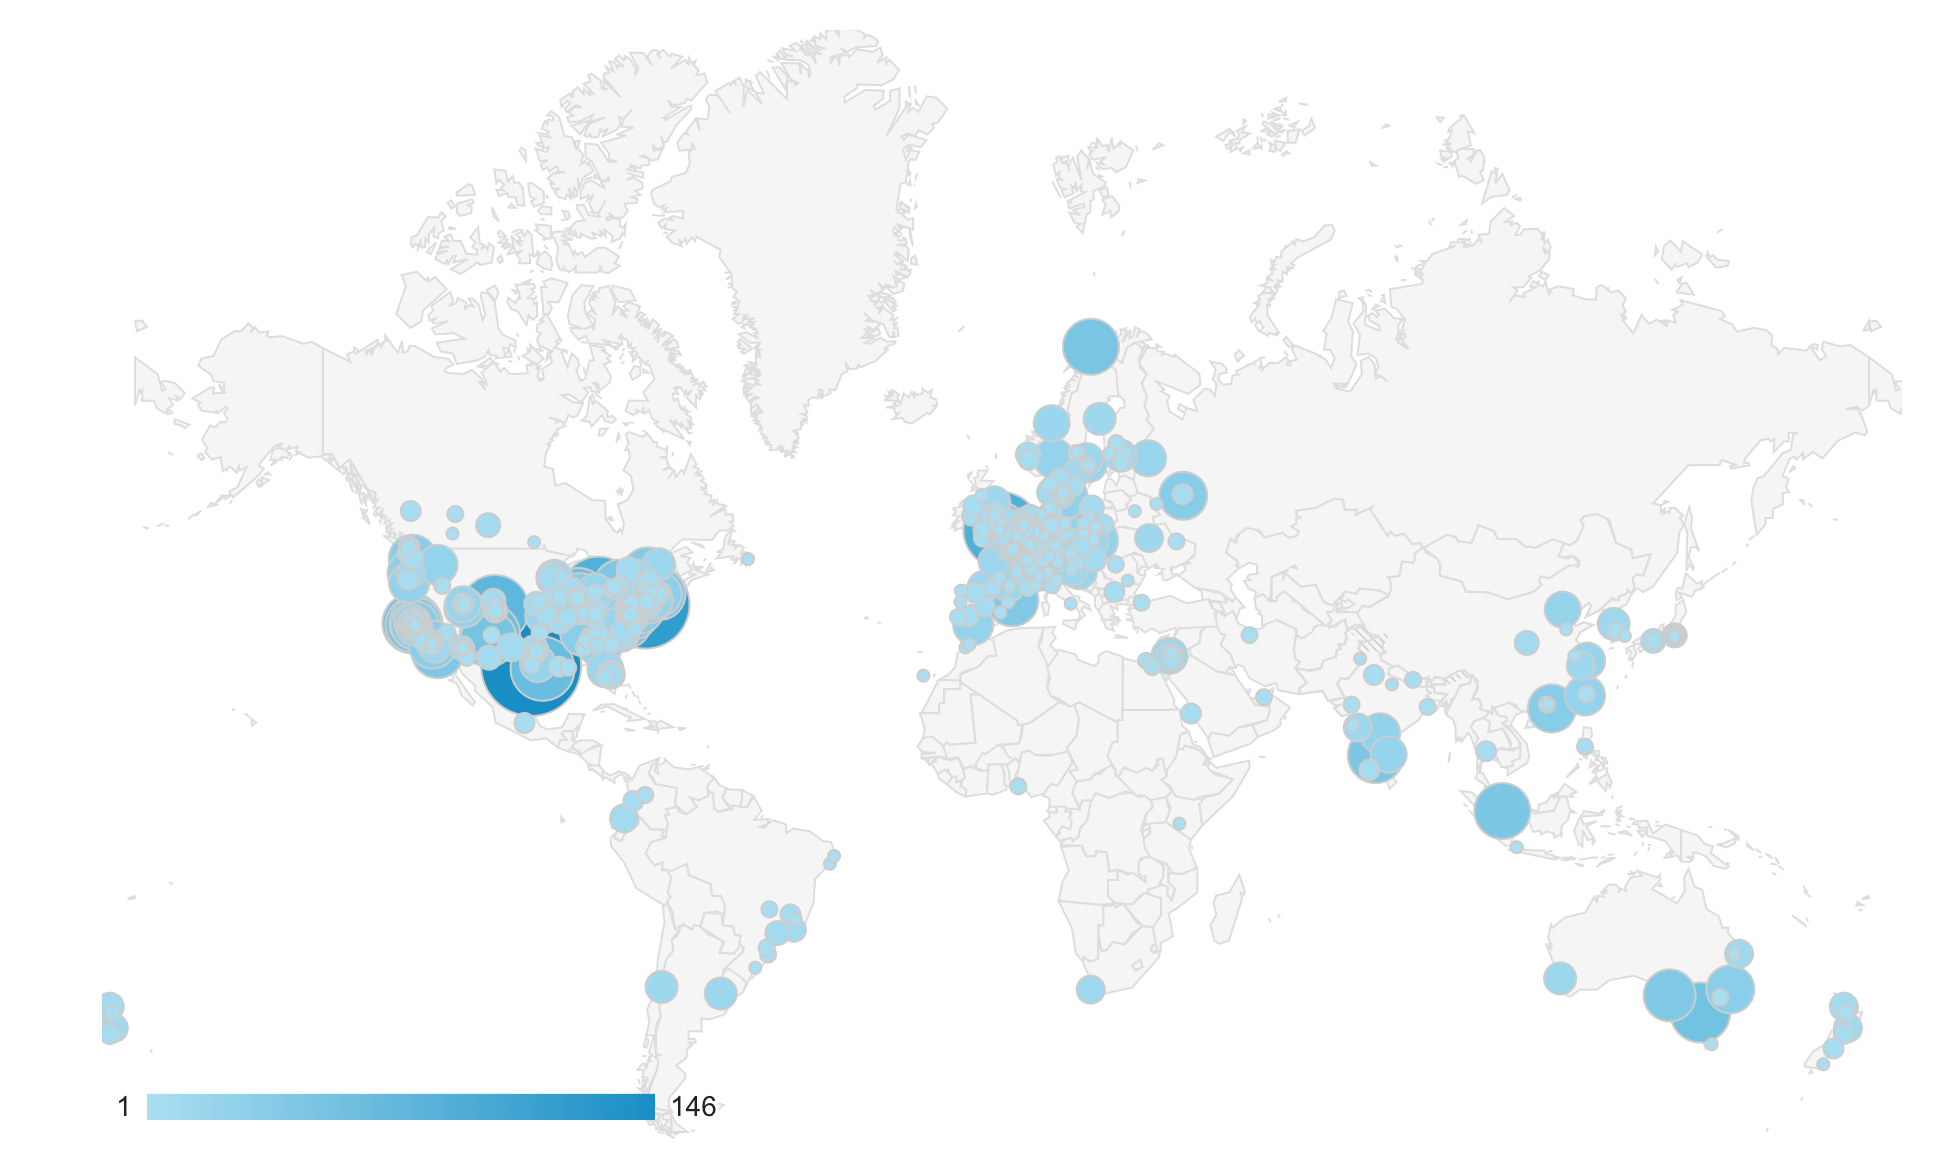
\includegraphics[width=.9\textwidth]{Lmod_docs_usage}}
\end{frame}


\begin{frame}{Other Talks of Interest at SC 18}
  \begin{itemize}
    \item BoF: Getting Software Installed Wed: 12:15 @ D175
    \item Vanderbilt U. \# 3727: Wed 11am, Thu. 2pm
    \item CEA \#2004 Wed 10-12 ``Module Rendez-vous''
    \item XALT @ NVIDIA \#2417 Wed 3:30
  \end{itemize}
\end{frame}

\begin{frame}{Conclusions: Lmod 7+}
  \begin{itemize}
    \item Latest version: https://github.com:TACC/Lmod.git
    \item Stable version: http://lmod.sf.net
    \item Documentation:  http://lmod.readthedocs.org
    \item This Talk: lmod.sf.net Presentations/SC18\_TACC\_Booth\_Lmod\_talk.pdf
  \end{itemize}
\end{frame}

\end{document}
